%% GENERATED FILE -- do not edit.
%% Written by scripts/manuscript/to_latex.py from manuscript/MANUSCRIPT_BMB_v5.md.
%% The markdown is the source; every number in it is recomputed by a script in
%% scripts/ and asserted by tests/.
%%
%% CLASS: Springer Nature sn-jnl, vendored at manuscript/springer/sn-jnl.cls
%% (LPPL). The option is sn-mathphys-ay -- AUTHOR-YEAR, which is what Bulletin of
%% Mathematical Biology uses and how the reference list below is written. The
%% Springer template ships with sn-mathphys-num uncommented; selecting it would
%% silently reformat the reference list into numbered style and break every
%% in-text citation, which are author-year throughout.
\documentclass[pdflatex,sn-mathphys-ay]{sn-jnl}

%% the class loads fontenc, geometry, hyperref, natbib, amsthm and others itself
\usepackage{amsmath,amssymb}
\usepackage{graphicx}
\usepackage[export]{adjustbox}
\usepackage{booktabs}
\usepackage{longtable}
\usepackage{array}
\usepackage{textcomp}
\usepackage{newunicodechar}
%% pandoc marks an uncaptioned longtable with \LTcaptype{none}; the caption
%% package then tries to step a counter of that name. Declaring it makes the
%% marker the no-op pandoc intends rather than a fatal error.
\newcounter{none}

\setlength{\emergencystretch}{3em}
\providecommand{\tightlist}{%
  \setlength{\itemsep}{0pt}\setlength{\parskip}{0pt}}

%% unicode that survives into prose, mapped from this document's own inventory
\newunicodechar{°}{$^\circ$}
\newunicodechar{±}{$\pm$}
\newunicodechar{²}{$^{2}$}
\newunicodechar{³}{$^{3}$}
\newunicodechar{¹}{$^{1}$}
\newunicodechar{×}{$\times$}
\newunicodechar{é}{\'{e}}
\newunicodechar{ö}{\"{o}}
\newunicodechar{Δ}{$\Delta$}
\newunicodechar{β}{$\beta$}
\newunicodechar{κ}{$\kappa$}
\newunicodechar{σ}{$\sigma$}
\newunicodechar{–}{--}
\newunicodechar{⁰}{$^{0}$}
\newunicodechar{⁴}{$^{4}$}
\newunicodechar{⁵}{$^{5}$}
\newunicodechar{⁶}{$^{6}$}
\newunicodechar{⁷}{$^{7}$}
\newunicodechar{⁸}{$^{8}$}
\newunicodechar{⁹}{$^{9}$}
\newunicodechar{⁺}{$^{+}$}
\newunicodechar{⁻}{$^{-}$}
\newunicodechar{→}{$\to$}
\newunicodechar{∎}{$\square$}
\newunicodechar{−}{$-$}
\newunicodechar{√}{$\surd$}

\title[Fold condition for quality-control models]{An Exact Fold Condition for Mass-Balanced Models
       of Protein Quality Control}
\author*[1]{\fnm{Kiran} \sur{Boggavarapu}}\email{kiran@mcneese.edu}
\affil*[1]{\orgdiv{Department of Chemistry and Physics}, \orgname{McNeese State University}, \orgaddress{\city{Lake Charles}, \state{LA}, \postcode{70609}, \country{USA}}}
\footnotetext{ORCID 0000-0003-0751-6459}

\abstract{A cell clearing misfolded protein with finite pools of chaperones and proteases tolerates damage influx only up to a threshold, beyond which burden runs away. Where that threshold sits is normally found by numerical continuation, one parameter set at a time. We show that it is algebraic. For any clearance network in which the damage influx is state-independent and mass balance accounts for all outflow, the Jacobian determinant factors as \(\det J = -(\nabla R \times \nabla G)\), where \(R\) is total removal flux and \(G\) the aggregate nullcline field. A fold therefore occurs exactly at a constrained critical point of removal on the aggregate nullcline, with critical influx \(j_{crit} = R(u^{*}, a^{*})\); the converse holds under four genericity conditions which we state and verify. The identity generalises to arbitrary state dimension, survives growth dilution, and survives clearance machinery that is itself damaged by the influx it clears. Three consequences follow. The fold occurs while the machinery runs at roughly 5--18\% of maximum velocity, so the capacity ceiling overestimates the tolerable influx about twelvefold. Under cell division the ceiling ceases to bound, and the critical influx decomposes exactly as \(j_{crit} = C_{enz}\cdot \varphi_{enz}/(1-\delta )\) with the enzymatic factor nearly invariant to division rate. When the machinery damages itself, a linear capacity ceiling becomes a square-root one. The fold is not always the first loss of stability: in a wide kinetic ensemble, 3.8\% of networks lose stability through a Hopf bifurcation first, in a region characterised by sharply saturating aggregate clearance against growth-dominated aggregation. Applied to the aggregation asymmetry of dividing \emph{Escherichia coli}, the framework yields a falsifiable requirement on the old-pole aggregate load as a function of the share held in the visible polar focus.}

\keywords{proteostasis, saddle-node bifurcation, conserved resource, clearance network, growth dilution, Hopf bifurcation}

\pacs[MSC Classification]{92C40 (primary); 37G10, 34C23, 92C42 (secondary)}

\begin{document}
\maketitle

\section{Introduction}

Protein quality control is a resource-limited clearance problem. Chaperones refold damaged monomers, proteases degrade them, and both draw on pools that are finite and shared across substrates (Hipp et al.~2019). Damage arrives continuously from translation error, thermal stress and oxidative modification. When influx exceeds what the machinery can dispose of, aggregate accumulates and the cell loses viability.

Models built on this premise locate the threshold numerically. One fixes a parameter set, integrates, continues the stable branch in the influx and records where it terminates. Cotton et al.~(2025) illustrate both the power and the cost of this approach: across eight variants of aggregate formation and removal kinetics they demonstrate that the same bifurcation structure is preserved, with a stable low-aggregate state and an unstable upper branch merging at a critical monomer concentration. The universality is established by exhibiting it case by case. Nothing in that treatment says why it should hold, or what would have to change for it to fail.

We show that for one structural class the threshold is algebraic rather than computational. Two facts about clearance models --- the damage influx enters one state equation, and mass balance is exact --- force the Jacobian determinant to factor into the cross product of two gradients. A fold is then a constrained critical point of total removal, in the Lagrange sense, on the nullcline of the non-influx equation, and the critical influx is the value of removal at that point. Adding states, adding regulation, adding cell division, or making the clearance capacity itself depend on the load leaves the identity intact.

The hypothesis required is weaker than it first appears. The theorem does not need influx and clearance capacity to be independent. It needs only that total influx be state-independent and that mass balance count all outflow. Capacity may depend on the error rate, on the burden, or on both. This matters because in a cell the chaperones and proteases are themselves translated by the error-prone apparatus whose product they clear.

Two results bound what the fold condition delivers. Solving the fold equations returns the candidate set exactly and without a sweep, but in about 9\% of a wide kinetic ensemble that set has more than one element, and identifying which candidate terminates the accessible branch requires information the equations do not carry. And the fold is not always the first loss of stability: in the same ensemble a Hopf bifurcation precedes it in a characterisable region of parameter space.

Section 2 fixes the model class and its hypotheses. Section 3 states and proves the fold condition, gives the genericity conditions for the converse, places the result relative to the homeostasis literature, and treats orientation and multiplicity. Section 4 gives three extensions. Section 5 reports numerical verification. Section 6 characterises where the fold sits relative to the capacity ceiling. Section 7 treats instabilities that precede the fold. Section 8 applies the framework to aggregation asymmetry in dividing \emph{E. coli}. Section 9 states what the theory predicts and what would refute it.

\section{The model class}

\subsection{State equations}

Let \(u\) denote damaged or misfolded soluble monomer and \(a\) aggregate burden, in compatible concentration units. The baseline field is

\begin{align*}
\frac{du}{dt} &= j - v_{ref}(u, C_f) - v_{degU}(u, D_f) - n(u) - g(u,a) + v_{dis}(a, C_f),\\
\frac{da}{dt} &= n(u) + g(u,a) - v_{dis}(a, C_f) - v_{degA}(a, D_f).
\end{align*}

with rate laws

\begin{align*}
v_{ref}  &= \frac{k_{ref}\,C_f\,u}{K_{ref} + u}   &&\text{refolding}\\
v_{degU} &= \frac{k_U\,D_f\,u}{K_U + u}           &&\text{soluble degradation}\\
n        &= k_n u^m,\quad m > 1                   &&\text{nucleation}\\
g        &= k_g\,u\,a                             &&\text{aggregate growth}\\
v_{dis}  &= \frac{k_{dis}\,C_f\,a}{K_{dis} + a}   &&\text{disaggregation}\\
v_{degA} &= \frac{k_A\,D_f\,a}{K_A + a}           &&\text{aggregate clearance}
\end{align*}

The two aggregate-forming terms are distinct processes. \(n = k_{n} u^m\) is primary nucleation with an effective reaction order greater than one, in the sense in which fitted orders are understood as coarse-grained descriptions of multi-step processes (Ferrone 1999; Knowles et al.~2009; Meisl et al.~2017). \(g = k_{g} u a\) is elongation: growth of existing aggregate at a monomer-dependent rate. The model as written carries no secondary nucleation term, which would be autocatalytic in aggregate surface (Cohen et al.~2013); adding one changes the coefficients below but not the structure, since it enters \(G\) and not \(R\).

Chaperone and protease pools are conserved and shared. Under rapid-equilibrium binding,

\begin{equation*}
C_f = \frac{C_{tot}}{1 + N_f/K_N + u_f/K_{CU} + a_f/K_{CA} + O_f/K_{CO}}
\end{equation*}

and similarly for \(D_{f}\), where \(N\) denotes nascent chains and \(O\) other competing substrates. The dissociation constants \(K_{CU}\) and \(K_{CA}\) describe competitive occupancy of the pool; the Michaelis constants \(K_{ref}\), \(K_{U}\), \(K_{dis}\), \(K_{A}\) describe the rate-limiting catalytic step that follows binding. The two are distinct steps and distinct constants. \(C_{f}\) is the pool not engaged in any complex, and the catalytic factor is the fraction of that pool turning over at the given substrate concentration. Nascent chains consume capacity without contributing damage influx, which is the mechanism by which ordinary translational load can move the fold.

Write the total removal flux and the aggregate field as

\begin{equation*}
R(u,a) = v_{ref} + v_{degU} + v_{degA},
\qquad
G(u,a) = \frac{da}{dt}
\end{equation*}

\(R\) is what leaves the damaged compartment; \(G\) is the non-influx equation. Note that \(n\) and \(g\) appear in \(R\) nowhere: they transfer material between \(u\) and \(a\) and cancel from \(du/dt + da/dt\). Aggregation does not oppose removal directly. It reshapes the nullcline, redistributes burden between the two pools, and suppresses effective removal through saturation and through sequestration of the shared machinery. Section 6 separates those two contributions.

\subsection{Hypotheses}

\textbf{H1 (state-independent influx).} The damage influx \(j\) is a parameter. It appears additively in \(du/dt\) and does not appear in \(da/dt\).

\textbf{H2 (exact mass balance).} Internal transfer between \(u\) and \(a\) cancels between the two equations, so \(du/dt + da/dt = j - R\) holds identically.

\textbf{H3 (smoothness).} \(R\) and \(G\) are continuously differentiable on the region of interest.

\textbf{H4 (deterministic, well-mixed, finite-dimensional).} The system is an ODE in concentrations.

\emph{Remark 1.} H1 constrains the influx, not the capacity. Nothing forbids \(C_{tot}\) or \(D_{tot}\) from depending on \(j\) or on the state. The gradients in Section 3 are taken at fixed \(j\), so parameter dependence on the influx cannot enter them, and the row operation requires only that \(j\) be additive in one equation and absent from the other. Corollary 4 treats the consequences of capacity that degrades with load.

\emph{Remark 2.} H4 is false in the system of Section 8 in two respects. Aggregates in \emph{E. coli} are spatially segregated into polar inclusion bodies rather than well mixed, and molecule numbers per damaged species are small. Both effects act in the same direction: noise-induced escape precedes the deterministic fold, so a measured threshold should sit below \(j_{crit}\) and be smeared across a population rather than sharp.

\section{The fold condition}

\subsection{The identity}

\textbf{Theorem 1.} \emph{Under H1--H3:}

\begin{enumerate}
\def\labelenumi{\arabic{enumi}.}
\tightlist
\item
  \emph{equilibria are exactly the points of the curve \(\{G = 0\}\) at which \(R = j\), and, when \(G\) does not depend on \(j\), that curve is independent of the influx;}
\item
  \(\det J = -(\nabla R \times \nabla G)\) \emph{identically;}
\item
  \emph{\(\det J = 0\) therefore holds exactly at constrained critical points of \(R\) restricted to \(\{G = 0\}\), where the critical influx is \(j_{crit} = R(u^{*}, a^{*})\).}
\end{enumerate}

\emph{Proof.} By H1, \(j\) appears in \(du/dt\) and nowhere in \(da/dt\), so \(\{G = 0\}\) is a curve in burden space on which the influx does not act; changing the load slides the state along it. An equilibrium requires \(G = 0\) and \(du/dt = 0\), and by H2 the second condition is \(R = j\) on that curve. This gives (1).

By H2, \(du/dt + da/dt = j - R\) exactly. The determinant-preserving row operation \(\operatorname{row}_{1} \to \operatorname{row}_{1} + \operatorname{row}_{2}\) gives

\begin{align*}
\det J
&= \det\begin{bmatrix}
     \partial(du/dt)/\partial u & \partial(du/dt)/\partial a\\[2pt]
     \partial(da/dt)/\partial u & \partial(da/dt)/\partial a
   \end{bmatrix}
 = \det\begin{bmatrix} -R_u & -R_a\\[2pt] G_u & G_a \end{bmatrix}\\[4pt]
&= -(R_u G_a - R_a G_u) = -(\nabla R \times \nabla G).
\end{align*}

which is (2). Vanishing of the determinant is \(\nabla R \parallel \nabla G\), the Lagrange condition for a critical point of \(R\) subject to \(G = 0\), and the equilibrium condition then gives the critical value. ∎

Informally: \textbf{the fold is where total removal stops responding to burden along the aggregate nullcline.}

At the base parameter set the alignment is visible rather than inferred: the removal contours meet the aggregate nullcline tangentially at the solved fold, to a sine of 3.54×10⁻¹⁰ (Fig. 1a). The same computed branch separates two singularities that are easily conflated. The soluble coordinate has a horizontal tangent at \(j_{turn} = 0.154090\), where \(G_{a} = 0\) and the nullcline runs vertical in the burden plane; that point is regular, since \(\det J = R_{a}\cdot G_{u} = 2.02749\times 10^{-3}\) there. The fold is at \(j_{crit} = 0.154239\), where both coordinates turn together (Fig. 1b). The two lie in a fixed order and differ by one part in a thousand. This is also why tracing \(\{G = 0\}\) by solving for \(a\) at fixed \(u\) fails: the two roots in \(a\) merge exactly at \(j_{turn}\), returning the curve in two disconnected pieces with the fold in the gap between them. The root-finder's failure and the horizontal tangent are one locus, not two problems.

\begin{figure}[htbp]
\centering
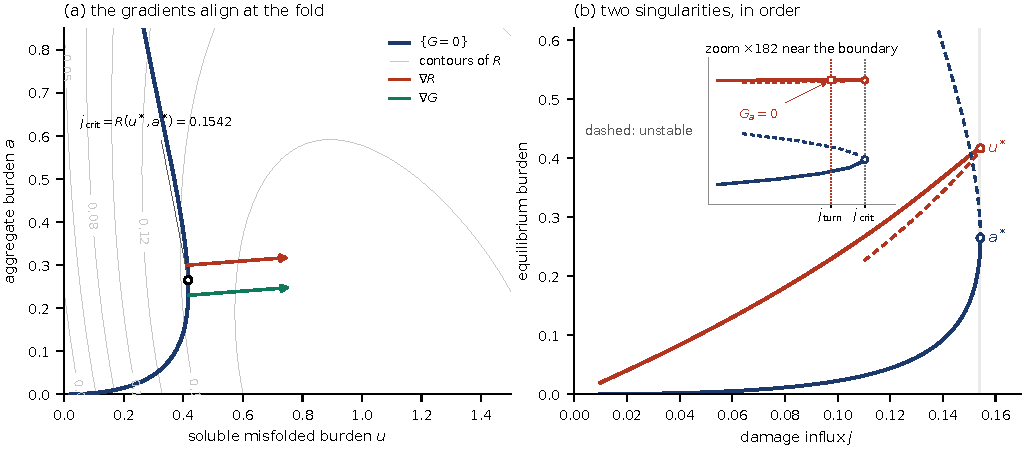
\includegraphics[max width=\linewidth]{../figures/fig1.pdf}
\caption{The fold as a constrained critical point. \textbf{(a)} Phase plane at the base parameter set. The aggregate nullcline $\{G = 0\}$ (dark) is fixed under change of influx; grey contours are total removal $R$. At the solved fold $(u^{*}, a^{*}) = (0.4166, 0.2650)$ the gradients $\nabla R$ and $\nabla G$ are parallel, which is the Lagrange condition of Theorem 1; they are drawn from offset origins because a common origin would hide one behind the other. The sine of the angle between them is 3.54×10⁻¹⁰, and $j_{crit} = R(u^{*}, a^{*}) = 0.1542$. \textbf{(b)} Both equilibrium coordinates against influx along the same curve. Cramer's rule gives $du^{*}/dj = -G_{a}/\det J$ and $da^{*}/dj = G_{u}/\det J$, so the branch carries two distinct, ordered singularities. At $j_{turn} = 0.154090$ the soluble coordinate has a horizontal tangent where $G_{a} = 0$; this is a regular point, $\det J = R_{a}\cdot G_{u} = 2.02749\times 10^{-3}$ there rather than zero, and it lies on the stable branch at $j_{turn}/j_{crit} = 0.9990$. At $j_{crit} = 0.154239$ both coordinates have a vertical tangent, which is $\det J = 0$. The inset is a ×182 zoom on the same computed data, not a schematic. The aggregate coordinate has no horizontal tangent anywhere: $G_{u} > 0$ at all 305 traced points, minimum 2.077×10⁻³.}
\label{fig:fig1}
\end{figure}

\subsection{Genericity, and the converse}

Theorem 1 gives one direction: a fold satisfies gradient alignment. The converse requires that the degeneracy be a fold rather than a transcritical or pitchfork bifurcation, a cusp, a double-zero eigenvalue, or a curve of equilibria. Four conditions suffice:

\begin{itemize}
\tightlist
\item
  \textbf{(G1)} regularity of the constraint, \(\nabla G \neq 0\);
\item
  \textbf{(G2)} a simple zero eigenvalue, \(\operatorname{tr} J \neq 0\);
\item
  \textbf{(G3)} nondegeneracy, \(d^{2}R/ds^{2} \neq 0\) along the nullcline at the critical point;
\item
  \textbf{(G4)} parameter transversality, \(w\cdot \partial F/\partial j \neq 0\) for the left null vector \(w\).
\end{itemize}

\textbf{Theorem 2 (converse).} \emph{Under H1--H3 and (G1)--(G4), a constrained critical point of \(R\) on \(\{G = 0\}\) is a generic saddle-node with \(j_{crit} = R(u^{*}, a^{*})\).}

(G4) is not automatic. Since \(\partial F/\partial j = (1, 0)\) exactly, transversality reduces to \(w_{1} \neq 0\), and no structural feature of the model forces it. Measured at solved fold states it is bounded away from zero: minimum 0.341 on the load grid and 3.34×10⁻⁹ over the kinetic box.

\textbf{Table 1} The four genericity conditions of Theorem 2, evaluated at every solved fold state in each ensemble. Each entry is the minimum of the condition's margin over the whole population; a value bounded away from zero means the condition holds throughout. The two exceptions are the same two networks in both rows where they appear.

\begin{table}[htbp]
\centering
\begin{tabular}{@{}lll@{}}
\toprule
condition & load grid (325) & kinetic box (2767) \\
\midrule
(G1) \(|\nabla G|\) & min 0.106 & min 1.04×10⁻⁸, 2 exceptions \\
(G2) \(|\operatorname{tr} J|\) & min 0.303 & min 8.38×10⁻⁴ \\
(G3) \(|d^{2}R/ds^{2}|\) & min 0.0929 & min 9.21×10⁻⁶ \\
(G4) \(|w_{1}|/|w|\) & min 0.341 & min 3.34×10⁻⁹, 2 exceptions \\
\bottomrule
\end{tabular}
\end{table}

The two exceptions are the same two networks, and they fail (G1), (G3) and (G4) together for one reason: both sit at aggregate burden of order 10⁻¹¹ and 10⁻¹⁵, where the aggregate compartment is empty, \(\nabla G \to 0\), the constraint ceases to be a manifold, and every condition defined on it degenerates. At both, \(\operatorname{tr} J = -\nabla R\) exactly, the signature of a state where \(G\) has gone flat. These are the boundary of the model's domain of definition rather than counterexamples to Theorem 2. A further 117 of 2884 sampled networks carry no solvable state satisfying \(\{G = 0, \det J = 0\}\) and are excluded from all conditions above.

Both computations use arclength along the nullcline rather than the \(u\)-coordinate. The nullcline turns vertical where \(G_{a} = 0\), which is a coordinate singularity of the \(u\)-parametrisation, and every quantity evaluated on the curve is affected there.

\subsection{Relation to infinitesimal homeostasis}

The hypotheses of Theorem 1 nearly coincide with those of an existing programme, and the relation is worth stating precisely.

Wang et al.~(2021) study input-output networks in which a parameter enters exactly one node's equation --- the condition H1 restates --- and ask when the input-output function \(x_{o}(I)\) has vanishing derivative. That question has a long history in the adaptation literature, where the stronger requirement of perfect adaptation demands the derivative vanish identically over an interval and the capable network topologies have been characterised numerically and then structurally (Ma et al.~2009; Ferrell 2016; Araujo and Liotta 2018; Khammash 2021). Cramer's rule applied to the implicitly differentiated equilibrium condition gives \(x'_{o} = \pm f_{\iota ,I} \det (H)/\det (J)\), where the homeostasis matrix \(H\) is the Jacobian with its first row and last column deleted. Infinitesimal homeostasis is \(\det (H) = 0\), and the programme built on that identity applies the Frobenius-König theorem to factor the determinant into irreducible blocks, each associated with a subnetwork motif of structural or appendage type (Golubitsky and Stewart 2017; Reed et al.~2017; Golubitsky and Wang 2020; Huang and Golubitsky 2022; Madeira and Antoneli 2024; Antoneli et al.~2025; Lin et al.~2026). The framework has since been extended to mass-action systems obeying conservation laws, using reduced Jacobian and reduced homeostasis matrices that incorporate the conserved quantities (Jin and Yu 2026).

The two conditions are complementary degeneracies of the same expression. Theirs is the vanishing of the numerator; ours of the denominator. Their derivation presupposes \(\det J \neq 0\), since the equilibrium is assumed hyperbolic, so the case Theorem 1 characterises is excluded from their setting by hypothesis. Geometrically, infinitesimal homeostasis is a horizontal tangent of the equilibrium branch in the input-output plane, where the output stops responding to the input; a fold is a vertical tangent, where the branch turns and the implicit function theorem fails. Neither condition implies the other.

Three degeneracies of the same equilibrium branch therefore arise: \(\det H = 0\) is homeostasis, \(\det J = 0\) with \(\operatorname{tr} J \neq 0\) is the fold, and \(\operatorname{tr} J = 0\) with \(\det J > 0\) is a Hopf bifurcation. This paper exhibits computed instances of the second and third (Sections 5 and 7) and a structural exclusion of the first. Taking the aggregate as output, the network is two nodes with a single arrow, \(H\) is 1×1, \(\det H = G_{u}\), and the only homeostasis type available is the degree-one Haldane form. It does not occur: \(G_{u} > 0\) throughout, because primary nucleation and elongation both rise with \(u\), and raising \(u\) also titrates chaperone and protease away from disaggregation and aggregate clearance, both of which enter \(G\) with a negative sign. All four contributions carry the same sign. Across 40 kinetic draws no traced point has \(G_{u} < 0\), the smallest value anywhere being 6.67×10⁻¹².

What makes our determinant factor differently is H2, which has no counterpart in the input-output setting. Mass balance supplies the row operation that replaces the influx row by \(-\nabla R\), so \(\det J\) factors into gradients of identified physical fluxes rather than into combinatorial blocks. Whether the combinatorial machinery transfers to \(\det J = -\det [\nabla R; \nabla G; \nabla C]\) is open; a Frobenius-König factorisation (Brualdi and Ryser 1991) of that determinant would classify fold mechanisms by network topology in the way structural and appendage blocks classify homeostasis mechanisms, and the decomposition of Section 6 is a two-term, physically motivated version of the same question.

The complementary question --- when regulation fails rather than when it holds --- was raised early in that literature and developed less. Nijhout et al.~(2014) ask what happens when a homeostatic mechanism is pushed past its range, and Reed et al.~(2018) treat homeostasis at equilibria that are not stable. Neither is a singularity-theoretic account of the failure. Theorem 1 supplies one for the case in which the failure is a fold.

The clearance-limited aggregation literature approaches the same object from the modelling side. Thompson et al.~(2021) analyse the stability of a minimal aggregate-removal model; Brennan et al.~(2023) treat clearance in a spatial setting; Cotton et al.~(2025) generalise to a phase-plane framework across eight aggregation and removal mechanisms, extracting two sufficient conditions for bistability and seeding --- self-replicating aggregation with a monomer-dependent rate, and limited-capacity removal. Their input parameter is the monomer concentration, which enters every term of both moment equations, so H1 fails for their system and Theorem 1 does not apply to it as stated. The model classes are adjacent rather than nested. What the present result adds within its own class is a derivation of why the bifurcation structure is preserved under extension, rather than a demonstration that it is.

\subsection{Orientation and multiplicity}

Two properties of the candidate set follow from the theorem and bound what it delivers.

\textbf{Orientation.} The sign of \(d^{2}R/ds^{2}\) distinguishes two kinds of fold. Where it is negative, \(R\) has a constrained local maximum, \(R = j\) has solutions below \(R(x^{*})\) and none above, and a pair of equilibria is destroyed as the influx rises: a collapse-oriented fold. Where it is positive, the pair is created as the influx rises: a birth-oriented fold, which is the lower turning point of a hysteresis loop rather than a collapse point. On the load grid \(d^{2}R/ds^{2} < 0\) at all 325 folds. Over the kinetic box, 26 of 2765 are birth-oriented, and all 26 carry a collapse-oriented candidate at strictly higher influx; 7 of 153 ordinary folds carry the same pair. Hysteresis is therefore a feature of the model class rather than of the 26. The operative consequence is that solving \(\det J = 0\) returns candidates without distinguishing them, so orientation must be computed and not inferred from a solver having converged.

\textbf{Multiplicity.} Neither \(G = 0\) nor \(\det J = 0\) contains \(j\), so locating candidates is a two-dimensional root solve rather than a continuation sweep in the influx.

\textbf{Corollary 1.} \emph{Solving \(\{G = 0, \det J = 0\}\) returns the candidate set exactly and without a sweep. Identifying which candidate terminates the accessible low-burden branch requires branch information in 9.1\% of the kinetic ensemble (252 of 2765 networks, up to five candidates).}

\section{Extensions}

\subsection{Arbitrary state dimension}

\textbf{Corollary 2.} \emph{Let the state be \(x = (u, a, c, \dots )\) with \(du/dt\) the only equation containing \(j\), and mass balance giving \(du/dt + da/dt = j - R(x)\). Writing the remaining equations as \(G\) and \(C\),}

\begin{equation*}
\det J = -\det\left[\,\nabla R \,;\, \nabla G \,;\, \nabla C\,\right]
\end{equation*}

\emph{which vanishes exactly when \(\nabla R\) lies in the span of the remaining gradients --- the Lagrange condition for a constrained critical point of \(R\) on the intersection of the non-influx nullclines. The converse requires, in addition to (G2)--(G4), that the non-influx constraint gradients have full rank.}

The proof is the same row operation on the first row of an \(n \times n\) Jacobian. The practical consequence is that a model in this class can be extended without re-deriving its fold condition.

We verify Corollary 2 on two three-state systems. In the first the chaperone pool is dynamical under σ32-style control, with synthesis rising as free chaperone falls: median relative error of the identity 0.000×10⁰ unregulated and 2.5×10⁻¹¹ to 2.9×10⁻¹¹ regulated, with the \(\sigma_{0} \to 0\) limit reproducing the two-state field exactly. In the second, aggregate is split into reactive and sequestered compartments: median 1.5×10⁻¹², maximum 4.7×10⁻¹¹ over a 144-point grid.

\subsection{Growth dilution}

Adding cell division leaves the theorem intact and removes the bound that made the capacity argument work.

Dilution does not affect binding, so the diluted field is \(du/dt - \mu u\), \(da/dt - \mu a\). H1 and H2 both survive, with total removal

\begin{equation*}
R_{tot} = R + \mu(u,a)\cdot(u + a)
\end{equation*}

so \(\det J = -(\nabla R_{tot} \times \nabla G_{dil})\) for any dilution law: verified at median relative error 1.2×10⁻¹⁰ for constant \(\mu\) and 4.7×10⁻¹⁰ for burden-dependent \(\mu\), with the \(\mu \to 0\) reduction exact. For constant \(\mu\) the diluted Jacobian is \(J - \mu I\), so the fold condition says exactly that \(\mu\) is an eigenvalue of the undiluted Jacobian.

The removal ceiling does not survive. \(R_{tot}\) contains \(\mu (u+a)\), unbounded in burden, so the bound \(j_{crit} \le C_{enz}\) fails once cells divide. At sufficiently large constant dilution the fold is destroyed outright: continuing in \(\mu\) at the base parameters gives \(j_{crit}\) rising 0.1542 → 0.2456 as \(\mu\) goes 0 → 0.08 while the fold state \(a^{*}\) diverges 0.265 → 0.750, and by \(\mu = 0.10\) no fold exists. Past that point the low-burden branch no longer terminates and burden rises smoothly with influx. Across 25 parameter draws having a fold at \(\mu = 0\), 23 lose it under constant dilution, at thresholds spanning 3.3 decades (p10/p50/p90 = 0.0033/0.086/0.328).

Burden-dependent growth restores it. With \(\mu (u,a) = \mu_{0}/(1 + (u+a)/k_\mu )\) a fold exists at every rate tested up to \(\mu_{0} = 0.3\). The physiological content is that burden-dependent growth reduction preserves the fold in a regime where constant dilution destroys it, not that division alone is incompatible with a fold.

The coupling itself is well established. Expressing protein a cell does not need reduces its growth rate, and the reduction scales with expression level (Dekel and Alon 2005; Shachrai et al.~2010). Coarse proteome partitioning makes the mechanism explicit: raising any sector's share comes at the expense of the ribosomal sector, and the resulting growth law predicts the burden of heterologous expression quantitatively (Scott et al.~2010, 2014; Scott and Hwa 2023). Calibrating against a measured dosage-response --- a 3.2\% growth rate reduction when misfolded protein represents less than 0.1\% of total cellular protein, measured in yeast (Geiler-Samerotte et al.~2011) and used here as a scaling assumption rather than a bacterial calibration --- gives slope 32 per unit misfolded proteome fraction and linear arrest at fraction 0.03125, both bounds rather than point values. Under this calibration a fold survives in 30 of 30 networks with \(\varphi_{enz}\) confined to 0.072--0.147.

Four properties must be distinguished and are not interchangeable: existence of a local fold; boundedness of total burden; genuine runaway; and crossing a viability threshold. The results above concern the first two.

\textbf{Corollary 3 (decomposition under division).} \emph{Splitting the critical influx into enzymatic and dilution parts,}

\begin{equation*}
j_{crit} = \frac{C_{enz}\,\varphi_{enz}}{1 - \delta},
\qquad
\varphi_{enz} = \frac{R_{enz}(u^{*},a^{*})}{C_{enz}},
\qquad
\delta = \frac{R_{dil}(u^{*},a^{*})}{j_{crit}}
\end{equation*}

\emph{with both factors dimensionless and in {[}0,1). The identity is algebraic and holds to 1.6×10⁻¹⁶.}

At the base parameters \(\varphi_{enz}\) stays within 0.125--0.134 as \(\mu\) runs 0 → 0.08, a ±4\% band, while \(\delta\) runs 0 → 0.39 and carries essentially all the variation. Division does not change the enzymatic condition for the fold; it multiplies the tolerable influx by \(1/(1 - \delta )\). Loss of the fold is \(\delta \to 1\), and across the draws above the median \(\delta\) at the threshold is 0.35: the fold is typically lost once division does about a third of the disposal work. Since growth rate is part of disposal, an experiment that lets growth rate float is not holding disposal capacity fixed. The two factors are drawn on one axis in Fig. 2 because the contrast is the content: \(\varphi_{enz}\) is flat to within 7.5\% of its own mean across the sweep while \(\delta\) traverses most of its range.

\begin{figure}[htbp]
\centering

\includegraphics[max width=\linewidth]{../figures/fig2.pdf}
\caption{Under division the enzymatic condition does not move; dilution does. A 33-point continuation at the base parameter set under constant dilution, plotted on one shared linear axis because the claim is a contrast between the two curves. Over $\mu$ from 0 to 0.080, $\varphi_{enz}$ stays within 0.1245–0.1343, a full width of 7.5\% of its own mean, while $\delta$ runs 0 to 0.3915 and carries essentially all the variation; $j_{crit}$ rises 0.1542 to 0.2456 and $a^{*}$ from 0.265 to 0.750. The band on $\varphi_{enz}$ is a complete enumeration over the sweep, not an extremum over a subsample. The Corollary 3 identity holds to p99 1.74×10⁻¹⁶ and maximum 1.77×10⁻¹⁶ across the sweep.}
\label{fig:fig2}
\end{figure}

\subsection{Self-damaging machinery}

In a cell, chaperones and proteases are translated by the error-prone apparatus, so raising \(j\) degrades the machinery that clears the damage.

We model this as \(C_{enz}(load) = C_0/(1 + \varepsilon \cdot load)\) applied to both pools, with \(\varepsilon\) swept over four decades in two modes: \(load = j\) and \(load = u + a\). The second places capacity inside \(\nabla R\) and \(\nabla G\) themselves.

The identity holds in both modes at machine precision: gradient-normalised residual with floor 2.2×10⁻¹⁴ at \(\varepsilon = 0\), and worst median 6.4×10⁻¹⁴ (influx mode) and 4.6×10⁻¹³ (burden mode) at \(\varepsilon = 100\), where capacity has fallen to 16.7\% and 1.8\% of nominal. No correction to the algebraic form is required, for the reason given in Remark 1: the row operation needs only that \(j\) be additive in \(du/dt\) and absent from \(da/dt\), and that \(du/dt + da/dt = j - R\) be exact.

What the coupling removes is the fixed nullcline. Under self-damage \(\{G = 0\}\) moves with the load, so \(j_{crit} = R(u^{*},a^{*})\) becomes a self-consistency condition and the candidate solve grows from two equations in \((u,a)\) to three in \((u,a,j)\). Corollary 1's saving applies to the frozen-capacity case.

Self-damage lowers the fold substantially without steepening the approach. Median \(j_{crit}\) relative to the frozen fold falls 0.999 / 0.990 / 0.925 / 0.640 / 0.322 across the influx ladder and 0.995 / 0.949 / 0.740 / 0.324 / 0.131 across the burden ladder. The critical-slowing exponent shows no detected shift: paired over the 19 networks carrying both values, median −0.4763 damaged against −0.4813 frozen, with a paired-difference distribution centred near zero (Wilcoxon \(p\) = 0.312).

\textbf{Corollary 4 (square-root capacity ceiling).} \emph{In influx mode every removal flux carries a factor \(1/(1 + \varepsilon j)\), so the necessary condition \(j \le C_0\) of the frozen model becomes \(\varepsilon j^{2} + j - C_0 \le 0\), that is}

\begin{equation*}
j \le \frac{\sqrt{1 + 4\varepsilon C_0} - 1}{2\varepsilon}
\;\longrightarrow\;
\sqrt{C_0/\varepsilon}
\quad\text{for large }\varepsilon.
\end{equation*}

A linear capacity ceiling becomes a square-root one: doubling the machinery buys only √2 in tolerable error rate once the machinery is itself error-prone. The bound is exact and is not binding in the range examined, with \(j_{crit}/j_{max}\) of median 0.039--0.186 and largest observed 0.623 over 8 draws, so it is a necessary condition and not the fold. Continuation with intermediate rungs recovers folds that a direct solve loses at large \(\varepsilon\), with recovery counts that do not decrease monotonically in \(\varepsilon\) (influx 7/5/6/6/4, burden 6/7/7/4/2); a genuine loss of the fold would be monotone, so this is continuation failure rather than folds disappearing. Where a fold does solve it satisfies \(\sin (\nabla R, \nabla G) < 2.0\times 10^{-9}\) throughout that sweep. The consequence is that Corollary 4 is least checkable numerically in the regime where it would bind.

\section{Numerical verification}

Two ensembles support the results. The \textbf{load grid} holds kinetics fixed at the base parameter set and sweeps nascent occupancy and rescue allocation, giving 325 folds; it describes how the fold moves within one network. The \textbf{kinetic box} is a Latin-hypercube ensemble of 5000 draws from a stipulated parameter box, of which 2884 admit a fold and 2767 yield a solvable fold state; it describes how the fold varies across networks. Every quantity below is recomputed from tracked generators and asserted by the accompanying test suite.

\textbf{Table 2} Numerical verification of the identity and the solver. Each row names its own ensemble because the two are not interchangeable, and each maximum is reported beside a p99 because a maximum grows with the size of the population it is drawn from while a p99 does not.

\begin{table}[htbp]
\centering
\begin{tabular}{@{}lllll@{}}
\toprule
quantity & ensemble & median & p99 & max \\
\midrule
identity residual, gradient-normalised & load grid, 325 & 2.34×10⁻¹⁰ & 9.67×10⁻¹⁰ & 1.29×10⁻⁹ \\
\(|G|\) at fold states & load grid, 325 & 4.95×10⁻¹⁴ & 9.40×10⁻¹⁰ & 1.63×10⁻⁹ \\
direct solver against continuation & load grid, 325 & 3.03×10⁻⁷ & 7.20×10⁻⁷ & 7.56×10⁻⁷ \\
\(\varphi\) rebuilt from first principles & kinetic box, 2884 & 1.3×10⁻¹³ & 2.98×10⁻⁹ & 7.25×10⁻⁹ \\
\bottomrule
\end{tabular}
\end{table}

Maxima over ensembles of different size are not directly comparable, and neither is comparable to a maximum computed at a third size; the p99 column is given for that reason, and at \(n = 325\) it rests on a small number of upper-tail observations.

The identity residual sits at the central-difference floor. The parallelism residual is not zero at recorded states and should not be: those are bracketed approximations whose leading eigenvalue is of order 10⁻⁴ rather than 0. The correlation between log parallelism error and log leading eigenvalue is +0.9960 over the load grid, showing the residual to be bracket tolerance rather than failure of the identity, and the tightest-bracketed state in the complete population has \(|\lambda |\) = 8.10×10⁻¹⁰ with \(\sin (angle)\) = 7.75×10⁻⁹ (Fig. S1).

One caution attaches to the self-damage check of Section 4.3. Because \(du/dt = j - R - G\) holds pointwise and the central-difference operator is linear, that check reproduces the row operation exactly at any step size and carries no truncation term; measured slopes in the step size are −0.97 and −0.94 with no minimum over four decades, which is roundoff alone. It certifies that the implementation preserves mass balance. The analytic argument carries the result.

\section{Where the fold sits}

Writing \(R = c_{f} s_{ref} + \rho_{U} d_{f} s_{u} + \rho_{A} d_{f} s_{a}\) against \(\operatorname{ceiling} = c_{tot} + \rho_{U} d_{tot} + \rho_{A} d_{tot}\), and \(\varphi = j_{crit}/\operatorname{ceiling}\), the saturation fractions at the fold answer how far below the ceiling it lies. The decomposition is evaluated at re-solved fold states satisfying \(\{G = 0, \det J = 0\}\) rather than where continuation stopped; of the 2884 draws admitting a fold, 2767 yield such a state and the remaining 117 are excluded and carry no entry. Evaluated instead at the recorded continuation states, \(\varphi\) reads 0.0806 and the ceiling factor thirteenfold rather than twelvefold.

\textbf{Table 3} Where the fold sits relative to the capacity ceiling, at re-solved fold states over the 2767 networks that admit one. The saturation fractions are Michaelis factors, so a value of 1 would mean the machinery is running at maximum velocity.

\begin{table}[htbp]
\centering
\begin{tabular}{@{}ll@{}}
\toprule
at the fold, kinetic box, 2767 solved states & median \\
\midrule
\(\varphi\) & 0.0825 \\
refolding saturation \(s_{ref}\) & 0.180 \\
soluble degradation saturation \(s_{u}\) & 0.159 \\
aggregate clearance saturation \(s_{a}\) & 0.049 \\
shortfall recovered by removing saturation & 35.9\% \\
shortfall recovered by removing sequestration & 12.6\% \\
\bottomrule
\end{tabular}
\end{table}

\textbf{The fold occurs while the clearance machinery runs at roughly 5--18\% of \(V_{max}\)}, so the capacity ceiling is a correct bound that overestimates the tolerable influx about twelvefold. That clearance saturation eventually fails to balance aggregation is the qualitative content of the limited-capacity condition identified by Cotton et al.~(2025); the decomposition above quantifies how far short of saturation the failure occurs, and splits it.

Two questions must not be merged. Saturation dominates the \emph{magnitude} of \(\varphi\); the \emph{existence} of a turning point requires the aggregation runaway that drives the free pools down at high burden. The counterfactuals answer the first only.

Dispersion is large. A nested design crossing 10 kinetic draws with a 7×7 load grid gives a between-to-within variance ratio for \(\varphi\) of 5.9, with per-network spread as large as 13.6× observed when both load coordinates sweep, against an 8.86× between-network spread --- so \(\varphi\) is network-characteristic but not load-invariant. The saturation box was chosen deliberately wide, so part of the between-network spread is a property of the sampling. Adding σ32-style regulation widens the p5--p95 width of \(s_{u}\) from 0.890 to 0.968 over the 30 networks of that experiment rather than narrowing it, with regulated median \(s_{u}\) 0.323 against 0.169 unregulated; only 14 of 30 regulated networks converged against 24 unregulated, so that comparison is indicative. Over the kinetic box the p5--p95 width of \(s_{u}\) is 0.867.

Fig. 3 shows why the dispersion, rather than the median, is what a reader should take from this section: the p5--p95 spans cover most of the unit interval, so a single measured saturation fraction discriminates weakly. Its inset gives the reason no screening floor is applied to the low-\(s_{a}\) tail --- the distribution runs smoothly across five decades with no gap, and the median slides continuously from 0.076 to 0.398 with whatever floor is imposed, so any floor is a free parameter moving a load-bearing number fivefold.

The claim this section supports is that the capacity bound overestimates by roughly an order of magnitude and that the fold is a computable constrained critical point --- not that the fold occurs at any particular fraction of \(V_{max}\).

\begin{figure}[htbp]
\centering
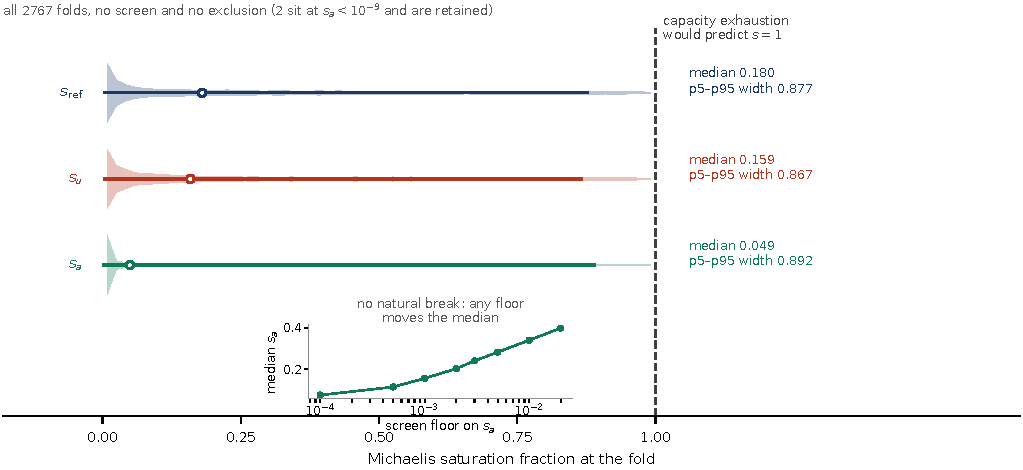
\includegraphics[max width=\linewidth]{../figures/fig3.pdf}
\caption{Saturation of the clearance machinery at the fold, over the 2767 kinetic-box networks that yield a solvable fold state, with none excluded. The distributions are evaluated at the same re-solved states as the table in Section 6, so figure and table describe one population; the p5–p95 widths are 0.877 for $s_{ref}$, 0.867 for $s_{u}$ and 0.892 for $s_{a}$. The point the figure carries is the width, not the centre: the spans are wide enough that a single measurement discriminates weakly against the capacity-exhaustion alternative. \textbf{Inset:} median $s_{a}$ against an imposed lower screening floor, from 0.076 at a floor of 10⁻⁴ to 0.398 at 2×10⁻². The distribution runs smoothly across five decades with no gap, so any floor is a free parameter that moves a load-bearing median by a factor of five. No floor is applied anywhere in this paper.}
\label{fig:fig3}
\end{figure}

\section{Instabilities preceding the fold}

The fold is not always the first loss of stability of the low-burden branch. Tracking \(\operatorname{tr} J\) along that branch from small \(j\) up to \(j_{crit}\), the load grid shows no crossing in any of its 325 networks, with \(\max (\operatorname{tr} J)\) of median −0.338 and largest −0.243. Over the kinetic box, 104 of 2766 networks --- 3.8\% --- reach \(\operatorname{tr} J = 0\) before the fold, with \(\det J > 0\) at the crossing in all of them (minimum 1.5×10⁻⁶), so the eigenvalues there are \(\pm i\sqrt\{\det J\}\). The first crossing occurs at a median of 0.83 of the way to \(j_{crit}\), with deciles 0.40 / 0.61 / 0.83 / 0.95 / 0.995.

A crossing network and a non-crossing one are traced together in Fig. 4a: the first rises through zero at about 0.82 of the way to \(j_{crit}\) and stays positive to the fold, while the second approaches the fold from below without ever reaching it.

Integration confirms the classification independently of the branch computation. Perturbing each of the 104 crossing networks at its own \(\operatorname{tr} J\) maximum, 104 grow by more than tenfold and 102 escape, with median \(\max |\delta |/\delta_{0}\) of 9851; 205 non-crossing networks perturbed at their own \(\operatorname{tr} J\) maximum give 0 escapes and median 1.00, with no overlap between the distributions (Fig. 4b). All 309 states are exact equilibria. The integration also recovers the eigenvalue: growth exponent within 5\% of \(\max Re(\lambda )\) in 90 of 104, and oscillation period within 5\% of \(\pi /\omega\) in 47 of 49.

The crossings occupy a coherent region of parameter space (Fig. 4c). Relative to non-crossing networks, aggregate clearance is faster (\(\rho_{A}\) 7.5× higher) and saturates more sharply (\(\kappa_{a}\) 11.7× lower), and aggregate formation is growth-dominated rather than nucleation-dominated (\(\alpha_{g}/\alpha_{n}\) shifting from 3.7 to 33.6, with \(\alpha_{g}\) alone only 1.67× higher). That configuration is a recognised destabilising one. Saturable rather than linear degradation of a reaction product lowers the cooperativity required for oscillation and, as the Michaelis constant of the degrading step falls, drives a stable steady state unstable (Goldbeter 2013); the same mechanism has been identified as the determinant of oscillation in NF-κB signalling, where strong saturation of IκB degradation destabilises the fixed point and weakening it restores stability (Krishna et al.~2006), and Michaelis-Menten degradation kinetics promotes oscillation across positive-feedback, negative-feedback and combined architectures (Xu and Qu 2012). Here the autocatalytic partner is elongation.

This is a distinct mechanism from the oscillation question in the regulated heat-shock response, which turns on transcriptional feedback and delay (El-Samad et al.~2005; Zheng et al.~2016; Sivéry et al.~2016). The networks above carry no regulation.

The incidence figure is a property of the stipulated parameter box and is not offered as a prediction. The load grid's cleanliness establishes that the base kinetic parameter set lies outside the oscillatory region, not that the region is small: the load grid holds kinetics fixed, and the crossing networks are distinguished by kinetic parameters.

\begin{figure}[htbp]
\centering
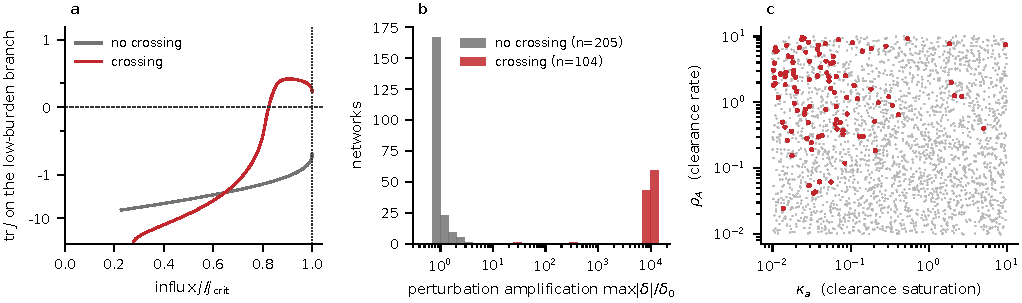
\includegraphics[max width=\linewidth]{../figures/fig4.pdf}
\caption{The fold is not always the first loss of stability. \textbf{(a)} $\operatorname{tr} J$ along the low-burden branch against $j/j_{crit}$, on a symmetric-log axis, for one crossing network and one non-crossing network. Both exemplars are chosen by rule rather than by inspection: the crossing case is the network nearest the median crossing position among those whose branch is resolved below 0.3 $j_{crit}$, and the non-crossing case is the network nearest the population median of $\max (\operatorname{tr} J)$. \textbf{(b)} Amplification of a perturbation applied at each network's own $\operatorname{tr} J$ maximum, integrating the full nonlinear system. The 104 crossing networks all grow by more than tenfold and 102 leave the linear neighbourhood, at a median amplification of 9851; the 205 non-crossing controls give 0 escapes and a median of 1.00. The distributions do not overlap. This panel shares no failure mode with the branch computation in (a). \textbf{(c)} Where the crossing networks sit in the sampled $(\kappa_{a}, \rho_{A})$ plane. Relative to the rest they have $\rho_{A}$ 7.5× higher and $\kappa_{a}$ 11.7× lower: clearance that is fast and sharply saturating.}
\label{fig:fig4}
\end{figure}

\section{Aggregation asymmetry in dividing *E. coli*}

Unstressed \emph{E. coli} accumulate aggregates at the old pole and lose reproductive capacity relative to new-pole progeny (Stewart et al.~2005; Lindner et al.~2008). Two features of the model class bear on this.

\subsection{What the model class cannot do}

No variant of the model examined places a stable attractor at low burden. Under constant dilution the system is bistable, with a 12.6- to 32.3-fold aggregate ratio between branches, but that regime predicts a growth-rate loss of exactly zero because \(\mu\) cannot respond to burden. Under the calibrated hyperbolic law the system is monostable in four of six settings tested. Under linear arrest there is no bounded high-burden state: \(\mu\) reaches exactly zero beyond \(k_\mu\), switching dilution off and removing the bound. Adding a sequestered compartment --- aggregate drained into an inert pool that neither nucleates nor occupies chaperone or protease --- produces 12 bistable cells against a control's 3, but none of 384 qualified cells predicts a loss within the measured range, every bistable cell predicting 0.482, 0.508, 0.954 or 1.000. Inverting the growth law, the high state is at least 7.5 to 254 times more aggregate-laden than the measured cell, and the upper figure is a lower bound because the 1.000 values are the linear-arrest law clamping at states 3.4 to 43 times past arrest. A real old-pole cell carries a visible inclusion body and divides at 96--99\% of normal.

\subsection{The observation does not require bistability}

The old-pole cell does not occupy a second basin. It inherits a physical inclusion body at each division, which is a continuously renewed perturbation rather than an attractor, and a monostable system under a renewed perturbation has a stationary offset with no separatrix.

The two-state diluted model under the calibrated hyperbolic law, with asymmetric partitioning of aggregate at division and no additional state variable, reproduces the measured lineage difference. Of 728 parameter settings, 709 settle, and 43 score within the measured range with the partitioning active. The control is exact: all 66 settings at symmetric partitioning give a lineage difference of 0.0 with standard deviation 0.0, which follows algebraically, since symmetric partitioning into half the volume leaves concentration unchanged and is what the \(-\mu x\) term already encodes.

\subsection{A requirement on the aggregate load}

The scored quantity is Lindner et al.'s \(\Delta (GR_{old} - GR_{new})/GR_{mean}\), whose aggregate-attributable part is 1.04--1.78\%, obtained from the reported lineage difference of −3.95 ± 0.5\% and the reported aggregate-attributable share of 30--40\%.

Partitioning is set by one physical quantity. The visible focus is indivisible and passes entirely to one daughter, but the model's \(a\) is total aggregate, of which the focus is a share \(\beta\). The old-pole daughter then receives \((1+\beta )a\) and the new-pole daughter \((1-\beta )a\) after division into half the volume, which is the scalar rule at \(f_{eff} = (1+\beta )/2\). With \(k_\mu = 0.03125/p_{qc}\), the scored quantity is \(32 \times (B_{old} - B_{new})\) as a proteome fraction exactly, so the quality-control proteome share and the growth rate enter only through the stationary load. Inverting gives a requirement scaling as \(1/\beta\):

\textbf{Table 4} The old-pole aggregate load required by the account of Section 8.3, as a function of the share \(\beta\) of aggregate held in the visible polar focus, over the same range Fig. 5 plots. The final column compares the requirement with the only aggregate load that has been measured, 5--10\% of total protein in Δ\emph{rpoH} at 30 °C; the columns pair the extremes, so they give the widest and narrowest separations consistent with both intervals.

\begin{table}[htbp]
\centering
\begin{tabular}{@{}llll@{}}
\toprule
\(\beta\) & \(f_{eff}\) & required old-pole aggregate (\% of proteome) & ratio to the Δ\emph{rpoH} load \\
\midrule
\(1.00\) & 1.000 & 0.047 -- 0.080 & 62× -- 214× \\
\(0.75\) & 0.875 & 0.061 -- 0.104 & 48× -- 165× \\
\(0.50\) & 0.750 & 0.091 -- 0.157 & 32× -- 110× \\
\(0.25\) & 0.625 & 0.182 -- 0.314 & 16× -- 55× \\
\(0.05\) & 0.525 & 0.913 -- 1.570 & 3.2× -- 11× \\
\bottomrule
\end{tabular}
\end{table}

The damping factor for the daughter's relaxation during its own generation is 0.346--0.355, with weak \(\beta\) dependence.

The table spans the same \(\beta\) range the figure plots. At \(\beta = 1.00\), where the whole aggregate is in the focus, the requirement sits 62× to 214× above the Δ\emph{rpoH} load; at \(\beta = 0.05\) it is 3.2× to 11× above it. Reporting only the rows down to \(\beta = 0.25\) would put the nearest approach at 16× and overstate the separation fivefold.

No source we could find bounds \(\beta\) under unstressed growth. Winkler et al.~(2010) report aggregate mass and focus size separately, and under heat stress, which is neither the condition at issue nor a focus-share measurement. The requirement is therefore a \(\beta\)-indexed family (Fig. 5), and the direction is the informative part: the less of the aggregate held in the focus, the more aggregate the account requires, and the closer the requirement moves to the only load anyone has measured. Tomoyasu et al.~(2001) report 5--10\% of total protein aggregated in Δ\emph{rpoH} mutants at 30 °C and no detectable aggregation in \emph{rpoH}⁺ cells at the same temperature; wild type is a bound rather than a value, and the reported mutant figures are not a limit of detection for the assay.

\begin{figure}[htbp]
\centering
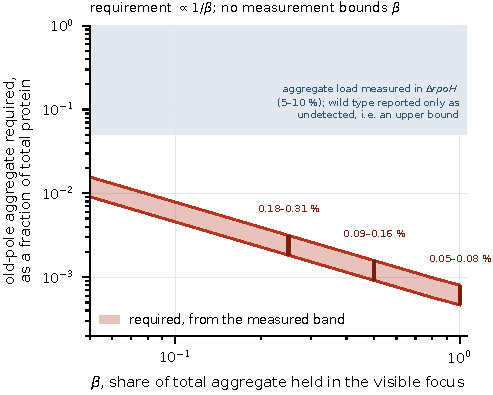
\includegraphics[max width=\linewidth]{../figures/fig5.pdf}
\caption{The old-pole aggregate load required by the account of Section 8.3, as a function of the focus share $\beta$, over the same range as the table there. The requirement scales as $1/\beta$: at $\beta = 1.00$ it is 0.047–0.080\% of the proteome and at $\beta = 0.05$ it is 0.913–1.570\%. The interval at each $\beta$ comes from the aggregate-attributable part of the measured lineage difference, 1.04–1.78\%. The shaded band is the only aggregate load anyone has measured, 5–10\% of total protein in Δ\emph{rpoH} at 30 °C; no measurement bounds $\beta$, so no vertical line is drawn.}
\label{fig:fig5}
\end{figure}

Two measurements close the question: the wild-type aggregate fraction under unstressed growth, and the share of that aggregate held in the polar focus, by quantitative fluorescence of the focus against total aggregated protein by sedimentation in the same cells.

\section{Predictions}

\textbf{Mathematical.} The identity \(\det J = -(\nabla R \times \nabla G)\), its \(n\)-state form, the converse under (G1)--(G4), the \(\mu \to 0\) and \(\sigma_{0} \to 0\) reductions, the \(J - \mu I\) form under constant dilution, the \((\varphi_{enz}, \delta )\) decomposition, and Corollary 4 follow from H1--H3 and no observation bears on them.

\textbf{The fold sits far below saturation.} The alternative is capacity exhaustion, in which the fold occurs as \(s \to 1\). The observable is a ratio, so testing it does not require absolute copies-per-cell calibration. Two cautions: the dispersion in \(s_{u}\) is wide (p5--p95 width 0.867 over the kinetic box), so a single measurement discriminates weakly, and adding regulation widens rather than narrows it.

\textbf{The fold moves under nascent load.} Since nascent chains consume chaperone capacity without contributing influx, raising the load of perfectly folding protein should lower the tolerable damage influx; a model handling the two loads independently predicts no shift. Direction was correct in 67 of 68 settings over a 100-fold ladder, with median shift 1.22×. Growth rate sets the load coordinate and contributes about 1.6× on its own against the \textasciitilde1.8× contrast expected, so the experiment requires externally fixed growth rate: chemostat or turbidostat, not batch culture.

\textbf{Oscillation before collapse.} In networks with fast, sharply saturating aggregate clearance against growth-dominated aggregation, damped oscillations should appear in aggregate burden as the damage influx rises, becoming sustained before any runaway. The predicted period is \(\pi /\omega\) with \(\omega = \sqrt\{\det J\}\) at the crossing, and the observable signature is that the amplitude grows while the mean burden remains low.

\textbf{A ruler, not a test.} Approaching the fold, relaxation time scales as \(\tau \sim (j_{crit} - j)^{(-1/2)}\) (fitted slope 0.5077, \(r^{2}\) = 1.0000). This is generic to folds, so confirming it selects this model over nothing in particular. Its use is as an instrument for locating the fold in an experiment that then asks whether the fold moves.

\textbf{The measurement the theory most wants.} Whether growth arrest under misfolding burden is complete or asymptotic. Under the hyperbolic form, dilution keeps bounding the high-burden state and loss of proteostasis is a reversible switch; under linear arrest, \(\mu\) reaches exactly zero and the high state is a runaway. The available dosage-response constrains the slope only below 0.1\% misfolded protein, about 1.5 decades below the arrest burden where the two forms diverge, so it cannot adjudicate. That single functional form decides whether losing proteostasis in a dividing cell is recoverable.

\section{Discussion}

The fold of a mass-balanced clearance network is not something one has to find by sweeping. Given the removal flux and the aggregate nullcline, it is where their gradients become parallel, and the critical influx is the removal flux evaluated there. The statement requires no fitted parameter, holds for any number of states, survives growth dilution, and survives capacity that degrades with the load it carries. Two things bound what it delivers: the candidate set can have more than one element, and the fold is not always the first loss of stability.

What it does not do is predict a number without measured parameters. The dispersion in \(\varphi\) across the kinetic ensemble is large enough, and wide enough after calibration and after adding regulation, that the quantitative predictions above are ratio comparisons rather than point predictions. This is a structural result rather than a predictive one.

Santra et al.~(2019) reach a tipping point in a proteostasis model by chaperone titration under cumulative damage, which is the same qualitative claim about how collapse arises. The present contribution is the exact flux-geometric condition for where it occurs, and the classification of what else can happen first.

The Hopf result identifies a regime worth looking for. Oscillatory dynamics of aggregate burden in a clearance network requires no regulatory circuit --- only fast, sharply saturating clearance against autocatalytic growth, which is the classical saturable-degradation destabilisation acting on an aggregation system. Whether real quality-control networks occupy that region is open, and Section 9 states the signature.

The prediction a reader can act on is Section 8.3. If the aggregate burden of an aging \emph{E. coli} old-pole cell falls outside the interval required at the measured focal share, the account of the aging asymmetry given here is wrong. Neither of the two measurements needed has been attempted as far as we can determine.

\begin{center}\rule{0.5\linewidth}{0.5pt}\end{center}

\section*{Data and code availability}

All analysis code, parameter configurations, and the test suite asserting every numerical quantity reported here are at https://github.com/khatvangi/proteostasis-law-theory under the MIT licence, archived at https://doi.org/10.5281/zenodo.21794565 (concept DOI, resolving to the latest version).

\section*{References}

Antoneli F, Golubitsky M, Jin J, Stewart I (2025) Homeostasis in input-output networks: structure, classification and applications. \emph{Math Biosci}. arXiv:2405.03861

Araujo RP, Liotta LA (2018) The topological requirements for robust perfect adaptation in networks of any size. \emph{Nat Commun} 9:1757.

Brennan GS, Thompson TB, Oliveri H, Rognes ME, Goriely A (2023) The role of clearance in neurodegenerative diseases. \emph{SIAM J Appl Math} S172--S198. doi:10.1137/22M1487801

Brualdi RA, Ryser HJ (1991) \emph{Combinatorial matrix theory}. Cambridge University Press, Cambridge.

Cohen SIA, Linse S, Luheshi LM, Hellstrand E, White DA, Rajah L, Otzen DE, Vendruscolo M, Dobson CM, Knowles TPJ (2013) Proliferation of amyloid-β42 aggregates occurs through a secondary nucleation mechanism. \emph{Proc Natl Acad Sci USA} 110:9758--9763.

Cotton MW, Goriely A, Klenerman D, Meisl G (2025) A universal phase-plane model for in vivo protein aggregation. arXiv:2511.18893

Dekel E, Alon U (2005) Optimality and evolutionary tuning of the expression level of a protein. \emph{Nature} 436:588--592.

El-Samad H, Kurata H, Doyle JC, Gross CA, Khammash M (2005) Surviving heat shock: control strategies for robustness and performance. \emph{Proc Natl Acad Sci USA} 102:2736--2741.

Ferrell JE (2016) Perfect and near-perfect adaptation in cell signaling. \emph{Cell Syst} 2:62--67.

Ferrone F (1999) Analysis of protein aggregation kinetics. \emph{Methods Enzymol} 309:256--274.

Geiler-Samerotte KA, Dion MF, Budnik BA, Wang SM, Hartl DL, Drummond DA (2011) Misfolded proteins impose a dosage-dependent fitness cost and trigger a cytosolic unfolded protein response in yeast. \emph{Proc Natl Acad Sci USA} 108:680--685.

Goldbeter A (2013) Oscillatory enzyme reactions and Michaelis-Menten kinetics. \emph{FEBS Lett} 587:2778--2784. doi:10.1016/j.febslet.2013.07.031

Golubitsky M, Stewart I (2017) Homeostasis, singularities and networks. \emph{J Math Biol} 74:387--407.

Golubitsky M, Wang Y (2020) Infinitesimal homeostasis in three-node input-output networks. \emph{J Math Biol} 80:1163--1185.

Hipp MS, Kasturi P, Hartl FU (2019) The proteostasis network and its decline in ageing. \emph{Nat Rev Mol Cell Biol} 20:421--435.

Huang Z, Golubitsky M (2022) Classification of infinitesimal homeostasis in four-node input-output networks. \emph{J Math Biol} 84:25.

Jin J, Yu PY (2026) Infinitesimal homeostasis in mass-action systems. \emph{J Math Biol}. doi:10.1007/s00285-026-02352-y

Khammash M (2021) Perfect adaptation in biology. \emph{Cell Syst} 12:509--521.

Knowles TPJ, Waudby CA, Devlin GL, Cohen SIA, Aguzzi A, Vendruscolo M, Terentjev EM, Welland ME, Dobson CM (2009) An analytical solution to the kinetics of breakable filament assembly. \emph{Science} 326:1533--1537.

Krishna S, Jensen MH, Sneppen K (2006) Minimal model of spiky oscillations in NF-κB signaling. \emph{Proc Natl Acad Sci USA} 103:10840--10845. doi:10.1073/pnas.0604085103

Lin X, Antoneli F, Wang Y (2026) Automated classification of homeostasis structure in input-output networks. \emph{Bull Math Biol}, article 113.

Lindner AB, Madden R, Demarez A, Stewart EJ, Taddei F (2008) Asymmetric segregation of protein aggregates is associated with cellular aging and rejuvenation. \emph{Proc Natl Acad Sci USA} 105:3076--3081.

Ma W, Trusina A, El-Samad H, Lim WA, Tang C (2009) Defining network topologies that can achieve biochemical adaptation. \emph{Cell} 138:760--773.

Madeira JLO, Antoneli F (2024) Homeostasis in networks with multiple inputs. \emph{J Math Biol} 89:17.

Meisl G, Michaels TCT, Linse S, Knowles TPJ (2017) Scaling behaviour and rate-determining steps in filamentous self-assembly. \emph{Chem Sci} 8:7087--7097.

Nijhout HF, Best J, Reed MC (2014) Escape from homeostasis. \emph{Math Biosci} 257:104--110.

Reed M, Best J, Golubitsky M, Stewart I, Nijhout HF (2017) Analysis of homeostatic mechanisms in biochemical networks. \emph{Bull Math Biol} 79:2534--2557.

Reed MC, Duncan W, Nijhout HF, Best J, Golubitsky M (2018) Homeostasis despite instability. \emph{Math Biosci} 300:130--137.

Santra M, Dill KA, de Graff AMR (2019) Proteostasis collapse is a driver of cell aging and death. \emph{Proc Natl Acad Sci USA} 116:22173--22178.

Scott M, Gunderson CW, Mateescu EM, Zhang Z, Hwa T (2010) Interdependence of cell growth and gene expression: origins and consequences. \emph{Science} 330:1099--1102.

Scott M, Klumpp S, Mateescu EM, Hwa T (2014) Emergence of robust growth laws from optimal regulation of ribosome synthesis. \emph{Mol Syst Biol} 10:747.

Scott M, Hwa T (2023) Shaping bacterial gene expression by physiological and proteome allocation constraints. \emph{Nat Rev Microbiol} 21:327--342.

Shachrai I, Zaslaver A, Alon U, Dekel E (2010) Cost of unneeded proteins in \emph{E. coli} is reduced after several generations in exponential growth. \emph{Mol Cell} 38:758--767.

Sivéry A, Courtade E, Thommen Q (2016) A minimal titration model of the mammalian dynamical heat shock response. \emph{Phys Biol} 13:066008.

Stewart EJ, Madden R, Paul G, Taddei F (2005) Aging and death in an organism that reproduces by morphologically symmetric division. \emph{PLoS Biol} 3:e45.

Thompson TB, Meisl G, Knowles TPJ, Goriely A (2021) The role of clearance mechanisms in the kinetics of pathological protein aggregation involved in neurodegenerative diseases. \emph{J Chem Phys} 154:125101.

Tomoyasu T, Mogk A, Langen H, Goloubinoff P, Bukau B (2001) Genetic dissection of the roles of chaperones and proteases in protein folding and degradation in the \emph{Escherichia coli} cytosol. \emph{Mol Microbiol} 40:397--413.

Wang Y, Huang Z, Antoneli F, Golubitsky M (2021) The structure of infinitesimal homeostasis in input-output networks. \emph{J Math Biol} 82:62.

Winkler J, Seybert A, König L, Pruggnaller S, Haselmann U, Sourjik V, Weiss M, Frangakis AS, Mogk A, Bukau B (2010) Quantitative and spatio-temporal features of protein aggregation in \emph{Escherichia coli} and consequences on protein quality control and cellular ageing. \emph{EMBO J} 29:910--923.

Xu L, Qu Z (2012) Roles of protein ubiquitination and degradation kinetics in biological oscillations. \emph{PLoS ONE} 7:e34616. doi:10.1371/journal.pone.0034616

Zheng X, Krakowiak J, Patel N, Beyzavi A, Ezike J, Khalil AS, Pincus D (2016) Dynamic control of Hsf1 during heat shock by a chaperone switch and phosphorylation. \emph{eLife} 5:e18638.

\end{document}
